\documentclass{article}
\usepackage{tikz}
\usepackage{graphicx}
\usetikzlibrary{positioning,shapes.geometric,arrows.meta}

% Macros the editor should expand in labels.
\newcommand{\yes}{yes}
\newcommand{\no}{no}
\newcommand\NN{\mathbb{N}}
\newcommand{\step}[1]{Step~#1}
\definecolor{brand}{HTML}{1F77B4}
\definecolor{soft}{rgb}{0.95,0.95,0.9}

\tikzset{
  >={Stealth[round]},
  box/.style={draw=brand, fill=brand!10, thick, minimum width=24mm,
              minimum height=8mm, align=center},
  choice/.style={box, diamond, aspect=2.2, fill=soft},
}

\begin{document}
Two pictures in one document: the first sits inside a \verb|\resizebox|.

\begin{figure}[ht]
  \centering
  \resizebox{0.8\linewidth}{!}{%
    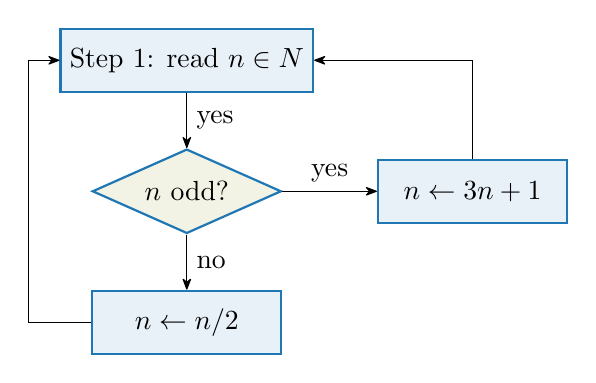
\begin{tikzpicture}[node distance=7mm and 12mm]
      \node[box]                (in)   {\step{1}: read $n \in \NN$};
      \node[choice, below=of in] (odd)  {$n$ odd?};
      \node[box, right=of odd]   (tri)  {$n \gets 3n+1$};
      \node[box, below=of odd]   (half) {$n \gets n/2$};
      \draw[->] (in) -- node[auto] {yes} (odd);
      \draw[->] (odd) -- node[above] {\yes} (tri);
      \draw[->] (odd) -- node[right] {\no}  (half);
      \draw[->] (tri) |- (in);
      \draw[->] (half.west) -- ++(-8mm,0) |- (in.west);
    \end{tikzpicture}%
  }
  \caption{Collatz step.}
\end{figure}

\begin{figure}[ht]
  \centering
  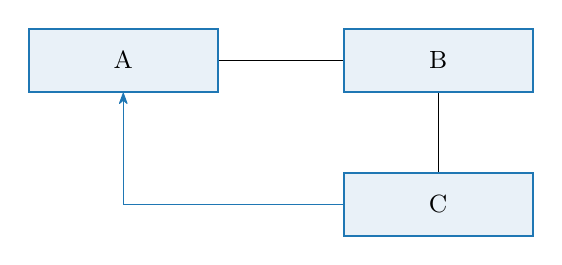
\begin{tikzpicture}[font=\small]
    \node[box] (a) at (0,0) {A};
    \begin{scope}[xshift=4cm, every node/.style={fill=brand!25}]
      \node[box] (b) at (0,0) {B};
      \node[box, below=of b] (c) {C};
    \end{scope}
    { [dashed]
      \draw (a) -- (b);
      \draw (b) -- (c);
    }
    \draw[->, brand] (c) -| (a);
  \end{tikzpicture}
  \caption{Scopes, in both forms.}
\end{figure}
\end{document}
